% Material found at https://www.elsevier.com/authors/author-schemas/latex-instructions

\documentclass{elsarticle}

\usepackage{lineno,hyperref}
\modulolinenumbers[5]

%=== Added for MU paper ====
\usepackage{color,soul} %% this was needed to have highlighted text
\usepackage{graphicx}
\usepackage{hyperref}
\usepackage{amsmath}
\usepackage{mathtools}
\usepackage{nomencl}
\makenomenclature
\graphicspath{{./figures/}}

\journal{Annals of Nuclear Energy}

%%%%%%%%%%%%%%%%%%%%%%%
%% Elsevier bibliography styles
%%%%%%%%%%%%%%%%%%%%%%%
%% To change the style, put a % in front of the second line of the current style and
%% remove the % from the second line of the style you would like to use.
%%%%%%%%%%%%%%%%%%%%%%%

%% Numbered
\bibliographystyle{model1-num-names}

%% Numbered without titles
%\bibliographystyle{model1a-num-names}

%% Harvard
%\bibliographystyle{model2-names.bst}\biboptions{authoryear}

%% Vancouver numbered
%\usepackage{numcompress}\bibliographystyle{model3-num-names}

%% Vancouver name/year
%\usepackage{numcompress}\bibliographystyle{model4-names}\biboptions{authoryear}

%% APA style
%\bibliographystyle{model5-names}\biboptions{authoryear}

%% AMA style
%\usepackage{numcompress}\bibliographystyle{model6-num-names}

%% `Elsevier LaTeX' style
%\bibliographystyle{elsarticle-num}
%%%%%%%%%%%%%%%%%%%%%%%

\begin{document}

\begin{frontmatter}

\title{Measuring Risk-Importance in a Simulation-Based PRA Framework}
%% \tnotetext[mytitlenote]{Fully documented templates are available in the elsarticle package on \href{http://www.ctan.org/tex-archive/macros/latex/contrib/elsarticle}{CTAN}.}

%% Group authors per affiliation:
\author{D. Mandelli, D. Maljovec, A. Alfonsi, C. Parisi, C. Smith}
\address{Idaho National Laboratory (INL), 2525 Fremont Ave, 83402 Idaho Falls (ID), USA}

\begin{abstract}
  Risk importance measures are indexes that are used to rank systems, 
structures and components (SSCs) using risk-informed methods. 
The most used/known measures are: Risk Reduction Worth (RRW), 
Risk Achievement Worth (RAW), Birnbaum (B) and Fussell-Vesely (FV). 
Once obtained from classical Probabilistic Risk Analysis (PRA) analyses, 
these risk measures can be effectively employed to relatively rank
component importance.
In contrast to classical PRA methods, 
Dynamic PRA methods couple stochastic models with safety analysis 
codes to determine risk associate to complex systems such as nuclear 
plants. Compared to classical PRA methods, simulation-based approaches
can evaluate with 
higher resolution the safety impact of timing and sequencing of events 
on the accident progression. 
The objective of this paper is to present a series of methods that 
can be employed to measure risk importance of components which are 
part of complex systems such as nuclear power plants.
The first set of measures are directly derived from classical risk 
importance measures (e.g., RRW, RAW, B and FV) and that can be employed
to any Dynamic PRA analysis.
In addition, we provide a set of risk importance measures that capture the 
dynamic nature of the problem and provide insight related to plant safety 
margins.

\end{abstract}

\begin{keyword}
%% keywords here, in the form: keyword \sep keyword
Data Mining \sep Dynamic PRA \sep Probabilistic Risk Assessment \sep Clustering 
\end{keyword}

\end{frontmatter}

\linenumbers

\printnomenclature[1in]

\section{Introduction}
\label{sec:introduction}
RAVEN (\textbf{R}isk \textbf{A}nalysis \textbf{V}irtual \textbf{EN}vironment)~\cite{Nureg1150}  is one of the many INL-developed software tools researchers can 
use to identify and 
increase the safety margin in complex systems (e.g. Nuclear Power Plants). It is a modular or ``plug-able'' framework that can be coupled with other computer 
modeling systems. RAVEN is capable to agnostically communicate with any system 
code. This agnosticism includes providing Application Programming Interfaces (APIs). These APIs are used to allow RAVEN to interact with any code as long as all 
the parameters that need to be perturbed are accessible through input files or via python interfaces. 
As a generic software framework, RAVEN is designed to perform parametric and probabilistic analysis based on the response of complex system codes. RAVEN is 
capable of investigating the system response as well as the input space using standard sampling techniques (e.g Monte Carlo, Grid, or Latin Hyper Cube), but its 
strength is focused toward system feature discovery, such as limit surfaces (i.e. separating regions of the input space leading to system failure, using dynamic 
supervised learning techniques), and advanced data analysis methodologies (i.e. Topology-based domain decomposition, Data Mining, Clustering, etc.).

The development of RAVEN has begun in 2012 to satisfy the need to provide a modern risk evaluation framework. RAVEN principal assignment is to provide the 
necessary software and algorithms in order to employ the concept developed by the Risk Informed Safety Margin Characterization (RISMC) path-
way~\cite{RISMC}. 
RISMC is one of the pathways defined within the Light Water Reactor Sustainability (LWRS) program. In the RISMC approach, the goal is not just specifically 
identifying the frequency of an event potentially leading to a system failure, but also to analyze the ``distance'' and the drivers toward the happening of key 
safety-related events. This approach may be used in identifying and increasing the safety margins related to those events. A safety margin is a numerical value 
quantifying the probability that a safety metric (e.g. as peak pressure in a pipe) is exceeded under certain conditions. The initial development of RAVEN has 
been focused on providing dynamic risk assessment capability to RELAP-7~\cite{RELAP7}, currently under development at the INL. All the methodologies
developed have been modularized in order to be applied to any computer modeling system (e.g., BISON, RELAP-7, RELAP5-3D, MELCOR, etc.).

The aim of this manuscript is to present a peculiar capability within the RAVEN framework named \textit{``EnsembleModels''}.

RAVEN is currently able to construct multi-targets Reduced Order Models (Ref.4), which are aimed to represent the response of a system (in a 
fixed configuration) for multiple Figures of Merits (FOMs) and time-dependent ROMs (see Ref.5). These capabilities represent the initial steps for a larger 
implementation about the interaction of multiple models. In fact, in several cases, multiple models need to interface with each other since the initial conditions of 
one are dependent on the outcomes of another.
To better understand the problem that here is solved, it is useful to consider two simple examples:
\begin{enumerate}
  \item The following problem is considered: a weather forecast simulation code ``a'' is used to compute the external (i.e. ambient) temperature in a certain location. 
  A second model ``b'' is inquired to compute the average temperature in a room having as boundary condition, among several others, the external ambient 
  temperature. The response of the model ``b'' depends on the outcome of the model ``a'';
   \item Two different simulation codes are considered: a) a code that is meant to compute the thermal conductivity of the ceramic Uranium Dioxide (UO2) as 
   function of the Temperature, and b) a Thermal-hydraulic (TH) code that is used to compute the Temperature field of a reactor, whose heat conduction depends on 
   the thermal conductivity value. As easily inferable, the two models are mutual dependent, determining in a non-linear system of equations.
\end{enumerate}
The two reported examples are only aimed to illustrate the reason why the creation of a framework to make interact different models is a key development for the 
advancement of RAVEN as a comprehensive calculation flow driver. Before reporting how the ensemble-models have been implemented, it is necessary to briefly 
describe the representative Model ``entities'' that are available in RAVEN.



\begin{figure}
    \centering
    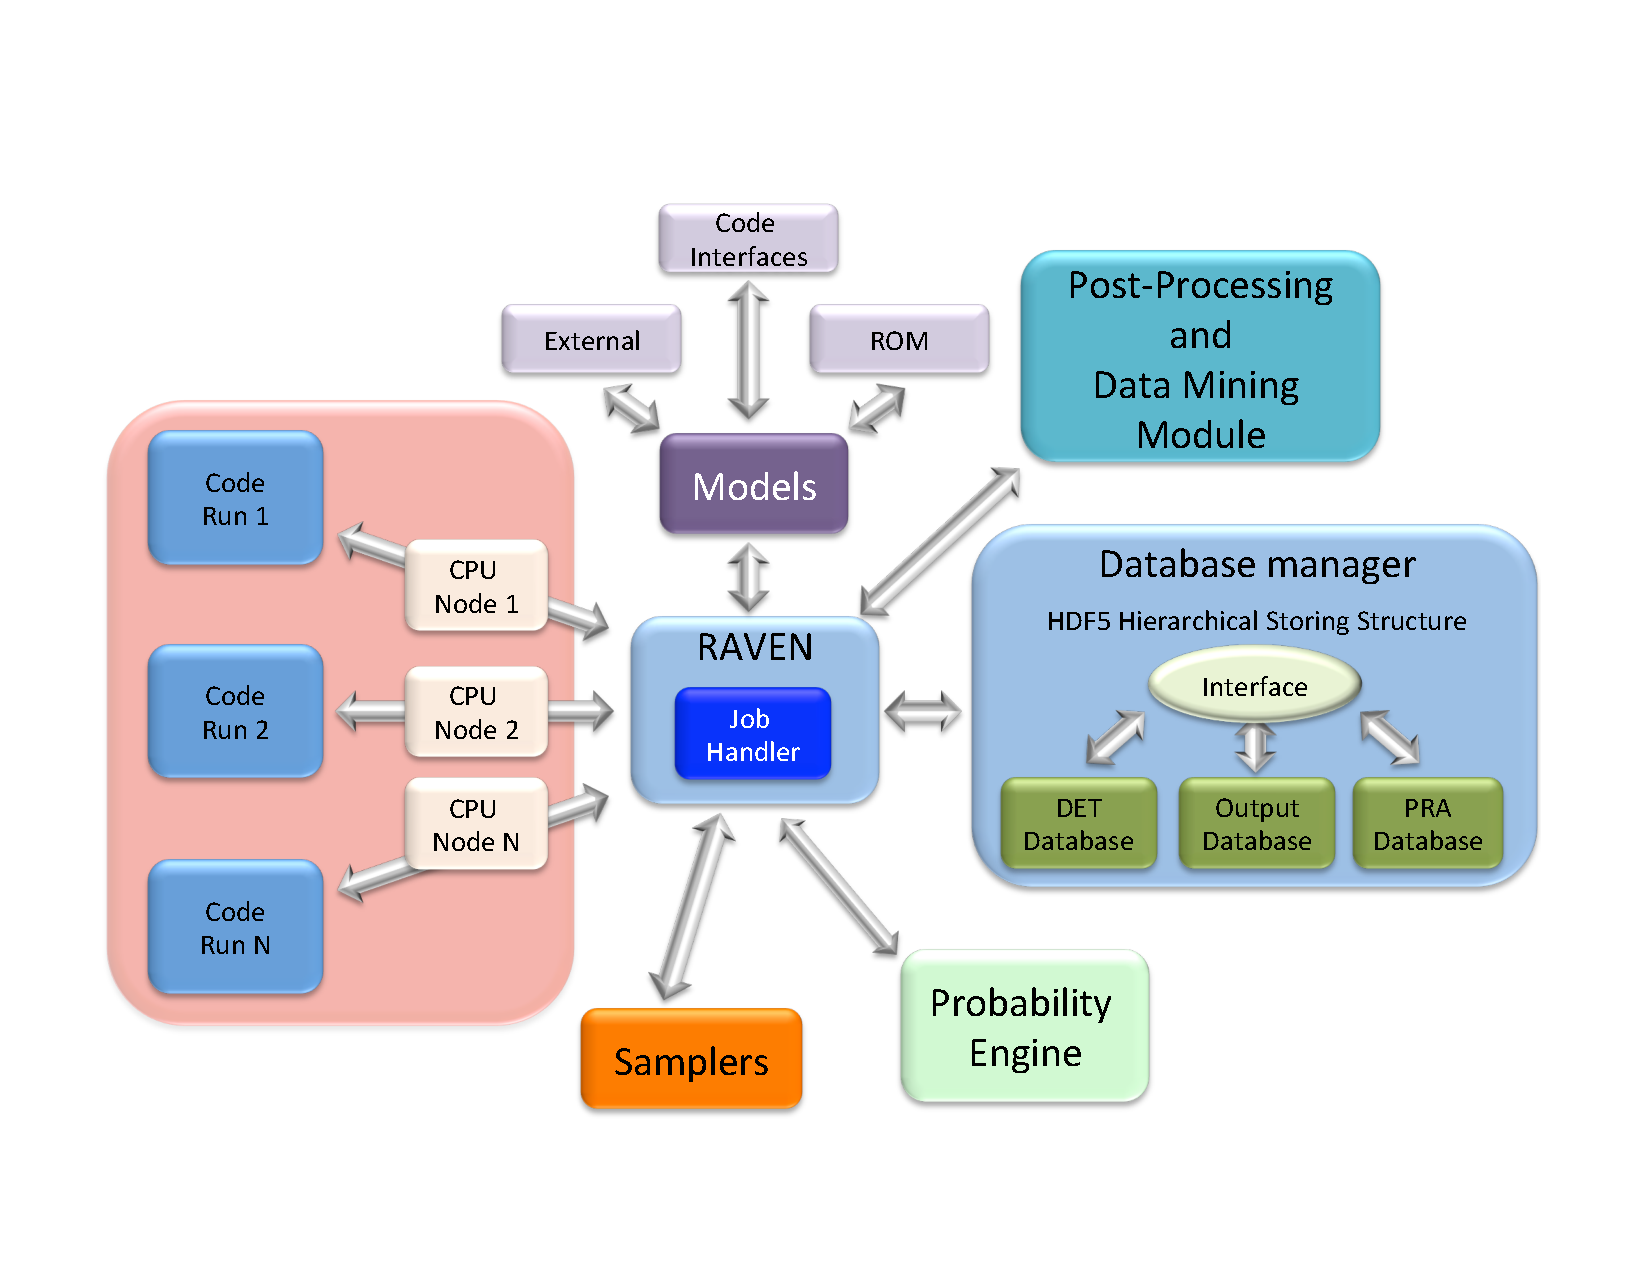
\includegraphics[scale=0.5]{raven.pdf}
    \caption{RAVEN}
    \label{fig:raven}
\end{figure}

\section{RISMC Approach to PRA}
\label{sec:rismc}

The RISMC approach~\cite{RISMC} employs both deterministic and stochastic methods 
in a single analysis framework (see Figure~\ref{fig:RISMCoverview}). In the deterministic method 
set we include:
\begin{itemize}
  \item Modeling of the thermal-hydraulic behavior of the plant~\cite{BWR_SBO_Mandelli,BWRanalysis}
  \item Modeling of external events such as flooding~\cite{mandelliPSA2015}
  \item Modeling of the operators’ responses to the accident scenario~\cite{HRA_BoringReport2014}
\end{itemize}

\begin{figure}
    \centering
    \centerline{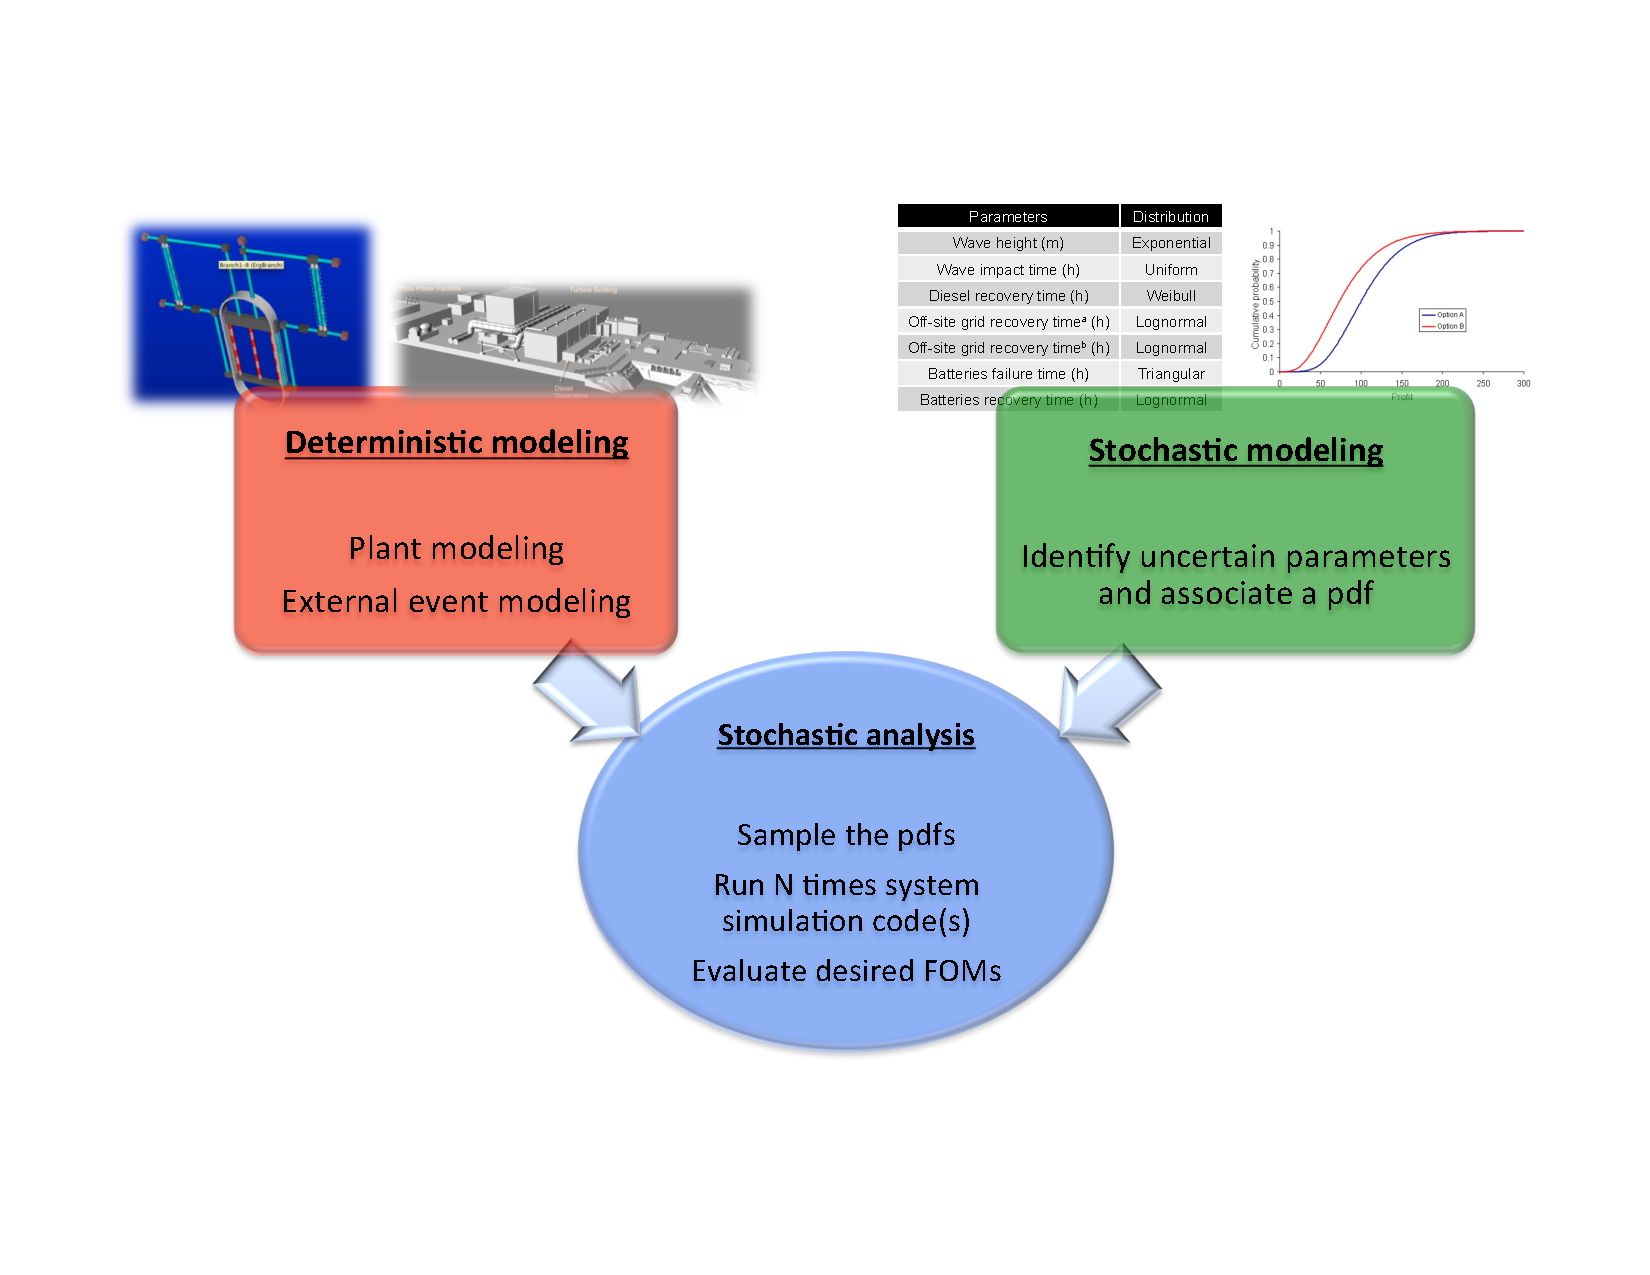
\includegraphics[scale=0.4]{RISMCoverview.pdf}}
    \caption{Overview of the RISMC approach}
    \label{fig:RISMCoverview}
\end{figure}

Note that deterministic modeling of the plant or external events can be performed by employing specific 
simulator codes but also surrogate models~\cite{ROM}, known as reduced order models (ROM). ROMs would 
be employed 
in order to decrease the high computational costs of employed codes. In addition, multi-fidelity codes 
can be employed to model the same system; the idea is to switch from low-fidelity to high-fidelity code 
when higher accuracy is needed (e.g., use low-fidelity codes for steady-state conditions and high-fidelity 
code for transient conditions)

In the stochastic modeling we include all stochastic parameters that are of interest in the PRA analysis 
such as uncertain parameters and stochastic failure of system/components.
As mentioned earlier, the RISMC approach heavily relies on multi-physics system simulator codes 
(e.g., RELAP5-3D~\cite{relap5}) coupled with stochastic analysis tools (e.g., RAVEN~\cite{raven}).  
From a PRA point of view, this type of simulation can be described by using two sets of variables:
\begin{itemize}
  \item $\boldsymbol c = \boldsymbol c(t)$ represents the status of components and systems of the simulator 
        (e.g., status of emergency core cooling system, AC system)
  \item $\boldsymbol \theta = \boldsymbol \theta (t)$ represents the temporal evolution of a simulated 
        accident scenario, i.e., $\boldsymbol \theta (t)$ represents a single simulation run. 
        Each element of $\boldsymbol \theta$ can be for example the values of temperature or pressure in 
        a specific node of the simulator nodalization.
\end{itemize}

From a mathematical point of view, a single simulator run can be represented as a single trajectory in the 
phase space. The evolution of such a trajectory in the phase space can be described as follows:
\begin{equation}
  \begin{cases}
    \dfrac{\partial \boldsymbol \theta }{\partial t}  = \boldsymbol \Xi (\boldsymbol \theta , \boldsymbol c, \boldsymbol s , t)   \\ \\ 
    \dfrac{\partial \boldsymbol c }{\partial t}  = \boldsymbol \Gamma (\boldsymbol \theta , \boldsymbol c, \boldsymbol s , t) 
  \end{cases}    
  \label{eq:trajectory}
\end{equation}
where:
\begin{itemize}
  \item $\boldsymbol \Xi$ is the actual simulator code that describes how θ evolves in time
  \item $\boldsymbol \Gamma$ is the operator which describes how c evolves in time , i.e., the status 
        of components and systems at each time step
  \item $\boldsymbol C$ is the set of stochastic parameters.
\end{itemize}

Starting from the system located in an initial state, $\boldsymbol \theta (t=0) = \boldsymbol \theta(0)$, 
and the set of stochastic parameters (which are generally generated through a stochastic sampling process), 
the simulator determine at each 
time step the temporal evolution of $\boldsymbol \theta (t)$. At the same time, the system control logic  
determines the status of the system and components $\boldsymbol c(t)$.
 
By using the RISMC approach, the PRA analysis is performed by~\cite{}:
\begin{enumerate}
  \item Associating a probabilistic distribution function (pdf) to the set of parameters 
        $\boldsymbol s$ (e.g., timing of events)
  \item Performing stochastic sampling of the pdfs defined in Step 1
  \item Performing a simulation run given $\boldsymbol s$ sampled in Step 2, i.e., solve the 
        system of equations~\ref{??}
  \item Repeating Steps 2 and 3 $M$ times and evaluating user defined stochastic parameters such 
        as core damage (CD) probability ($P_{CD}$).
\end{enumerate}

\section{RISMC Approach and Classical PRA}
\label{sec:analogy}

In order to better understand the results obtained in Section~\ref{sec:test} it is worth to illustrate 
a link between classical PRA and RISMC approach.
Let's consider a system that is composed by two components (i.e, A and B) in a series configuration where
each component has a failure probability (i.e., $p_A$ and $p_B$ respectively) as shown in Fig.~ref{}.

In a classical PRA framework such system can be modeled using a FT method that is composed by two basic events:
A failed and B failed.
System failure would be represented by a single ``AND'' gate that combine the two basic events as shown in 
Fig.~ref{}.

\begin{figure}
  \centering
  \begin{subfigure}{.5\textwidth}
    \centering
    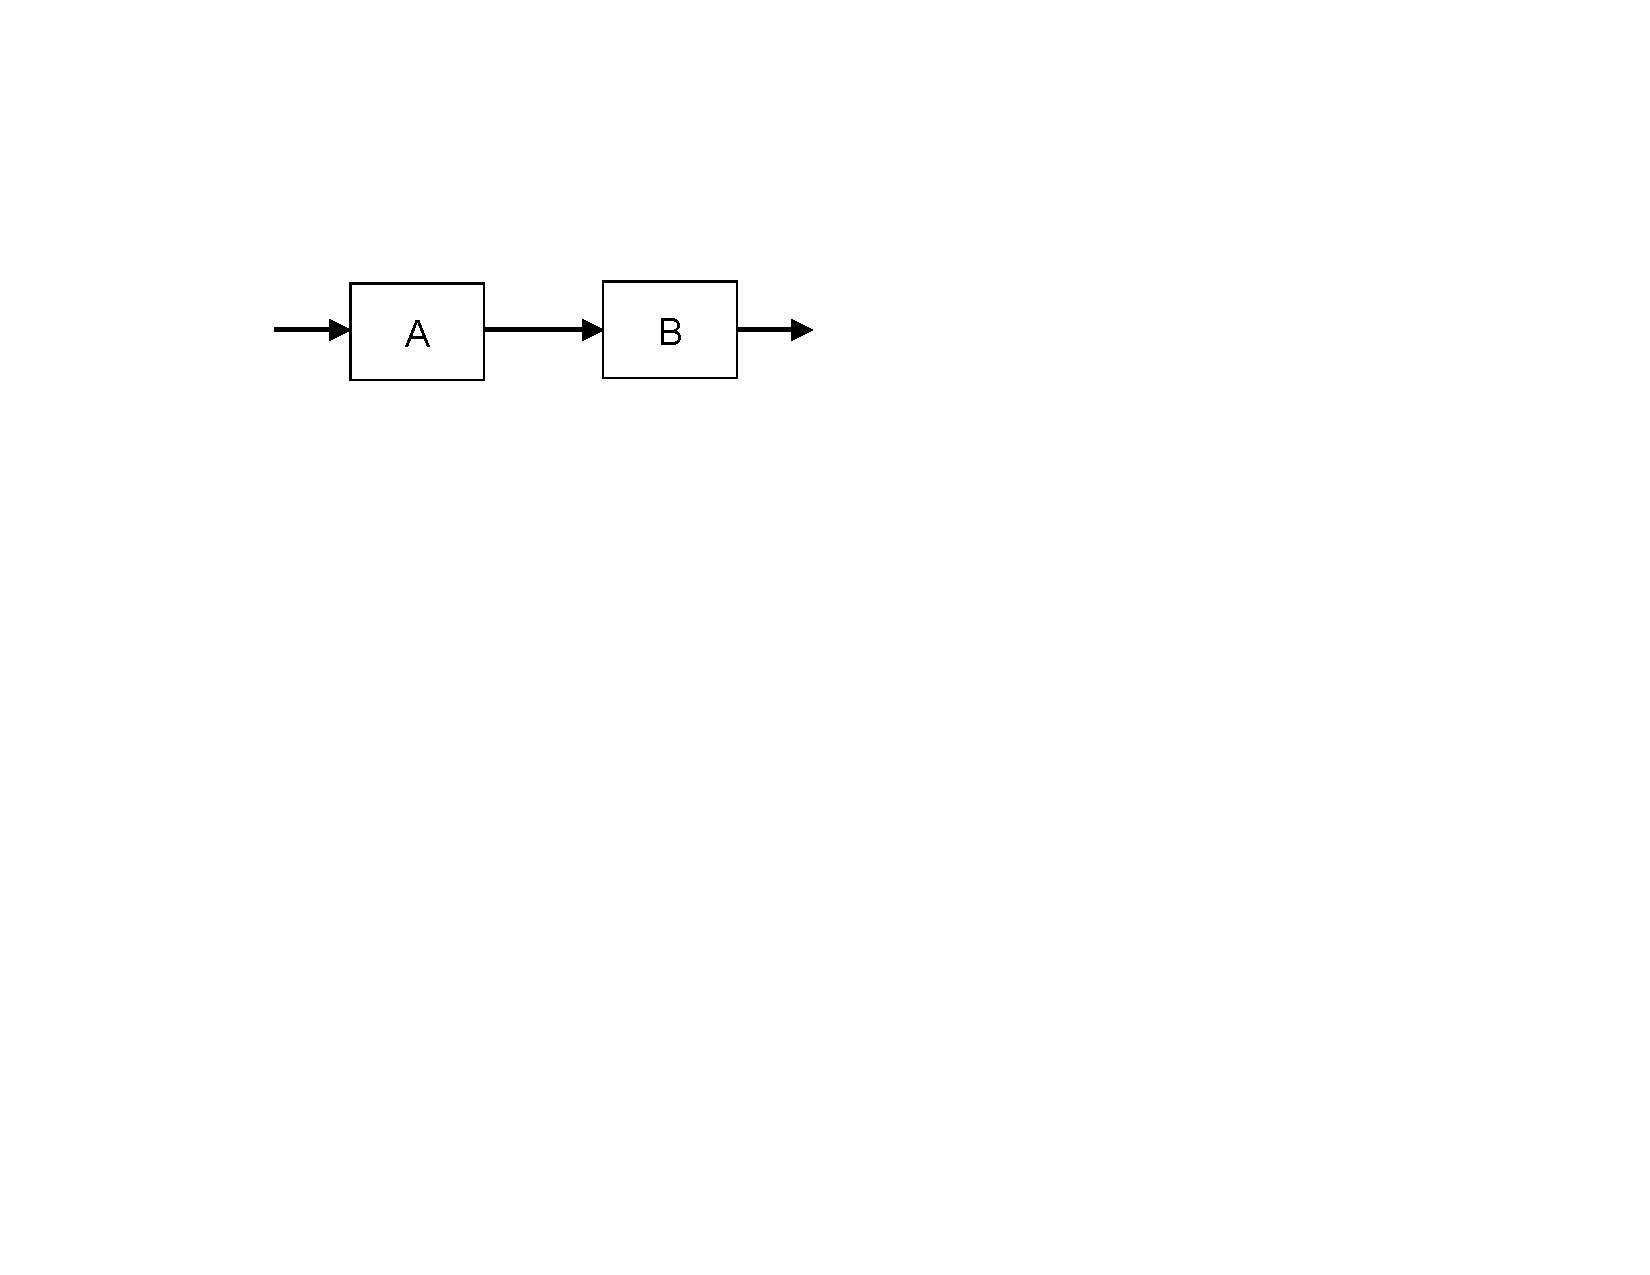
\includegraphics[scale=0.6]{ABsystem.pdf}
    \label{fig:sub1}
  \end{subfigure}%
  \begin{subfigure}{.5\textwidth}
    \centering
    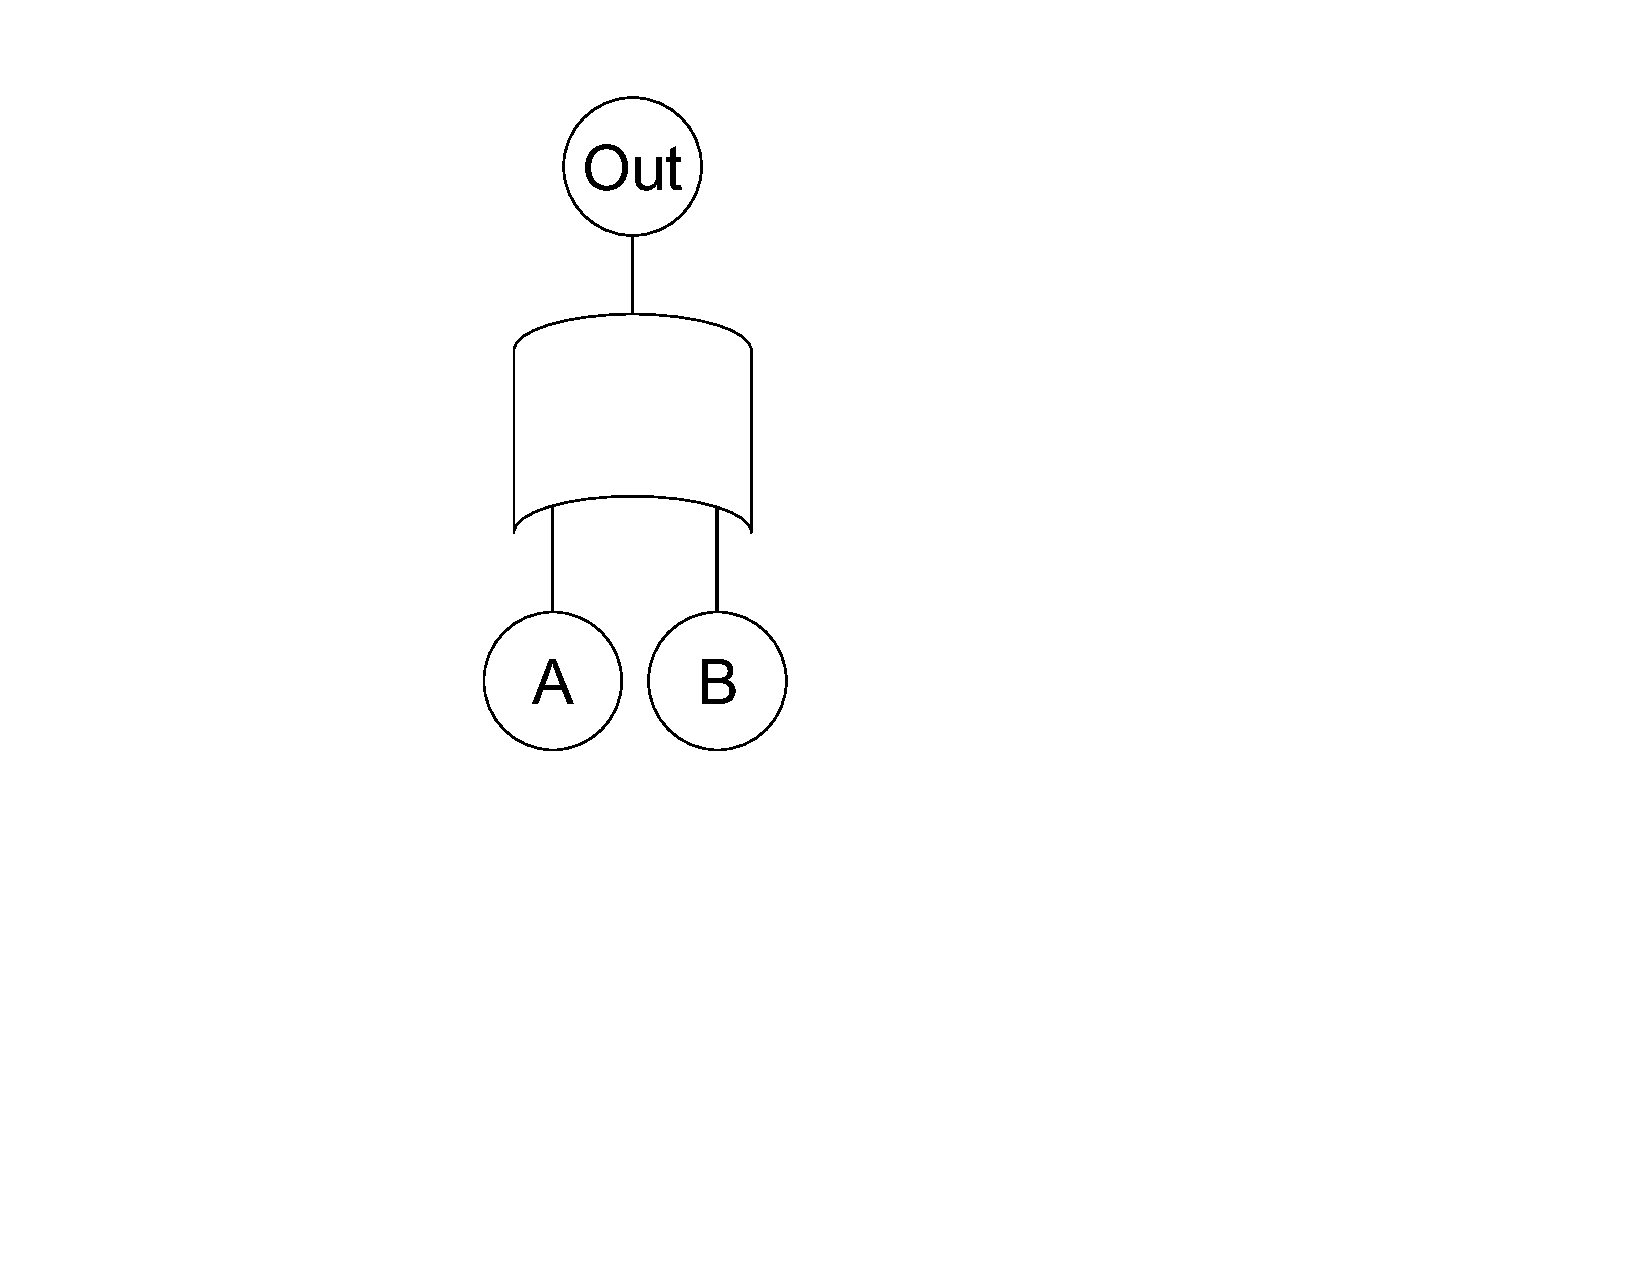
\includegraphics[scale=0.3]{andGate.pdf}
    \label{fig:sub2}
  \end{subfigure}
  \caption{Components A and B in a series configuration (left) and associated Fault-Tree (right).}
  \label{fig:chebyshev}
\end{figure}

\begin{figure}
    \centering
    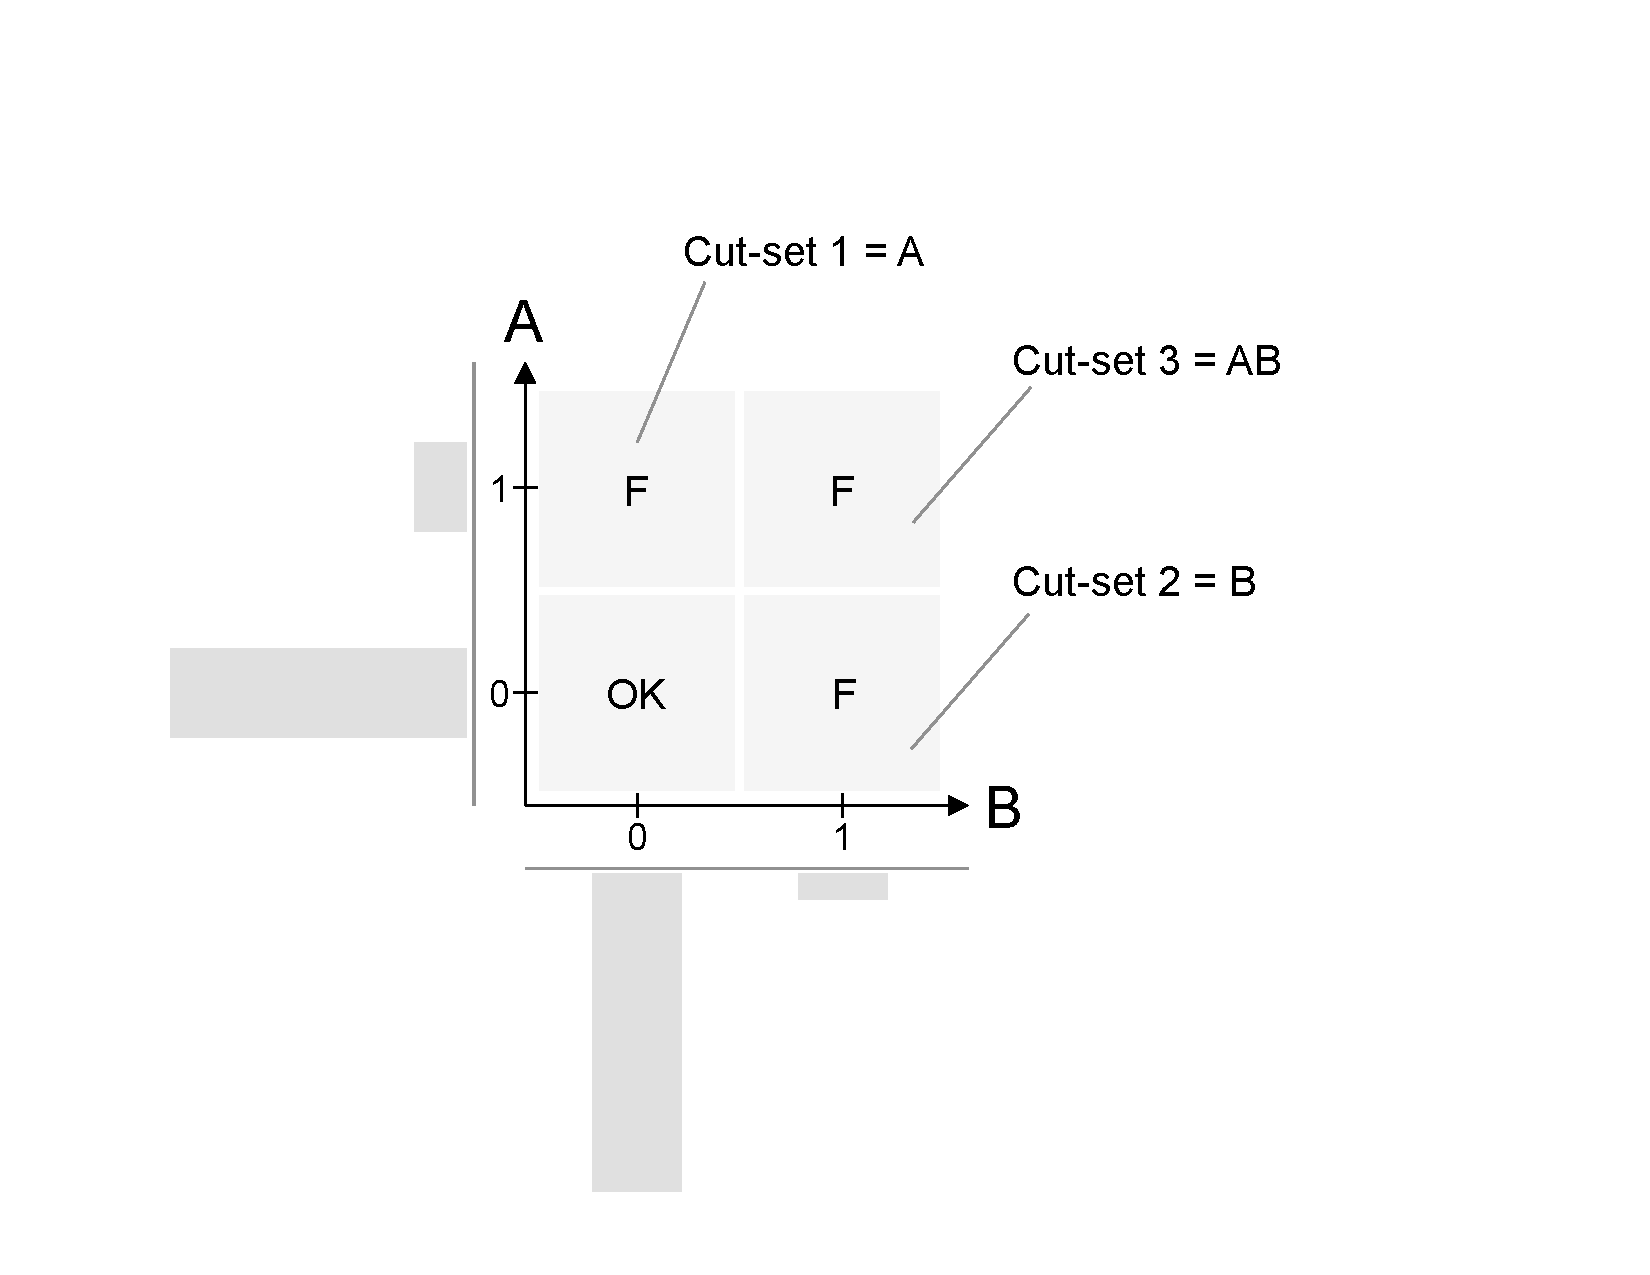
\includegraphics[scale=0.4]{2D.pdf}
    \caption{}
    \label{fig:2Danalogy}
\end{figure} 




\section{RAVEN}
\label{sec:raven}
 
The Risk Analysis and Virtual ENviroment 
(RAVEN\footnote{Official website: \url{https://raven.inl.gov},\\ 
GITHUB repository: \url{https://github.com/idaholab/raven}})
~\cite{RAVEN_PSAM_2014,alfonsiEsrel2014} 
is a flexible and multi-purpose uncertainty quantification, regression analysis, probabilistic
risk assessment, data analysis and model optimization framework. Depending on the tasks to be 
accomplished and on the probabilistic characterization of the problem, RAVEN perturbs 
(e.g., Monte-Carlo, latin hypercube, reliability surface search) the response of the system 
under consideration by altering its own parameters. The system is modeled by third party software 
(e.g., RELAP5-3D~\cite{relap5}, MELCOR~\cite{Melcor}) and accessible to RAVEN either directly 
(software coupling) or indirectly (via input/output files). 
The data generated by the sampling process is analyzed using 
classical statistical and more advanced data mining approaches. RAVEN also manages the parallel dispatching 
(i.e. both on desktop/workstation and large High Performance Computing machines) of the software 
representing the physical model. RAVEN heavily relies on artificial intelligence algorithms to construct 
surrogate models of complex physical systems in order to perform uncertainty quantification, reliability 
analysis (limit state surface) and parametric studies.

By statistical analysis we include:
\begin{itemize}
  \item Sampling of codes, either stochastic, e.g., Monte-Carlo~\cite{DynamicReliabilityMonteCarlo} 
        and Latin Hypercube Sampling (LHS)~\cite{LHShelton}, deterministic (e.g., grid and
        Dynamic Event Tree (DET)~\cite{AMENDOLAdylam,cojazziDylam}) or 
        adaptive~\cite{ANS_S_2014_raven_LS,mandelliSVMANS}
  \item Generation of ROMs~\cite{ROM_Khalik}, also known as Surrogate models
  \item Post-processing of the sampled data and generation of statistical parameters (e.g., mean, 
        variance, covariance matrix).
\end{itemize}

Figure~\ref{fig:ravenScheme} shows a general overview of the elements that comprise the RAVEN 
statistical framework:

\begin{itemize}
  \item Model: it represents the pipeline between input and output space. It comprises both codes 
        (e.g., RELAP5-3D~\cite{relap5}) and also ROMs 
  \item Sampler: it is the driver for any specific sampling strategy, e.g., Monte-Carlo, LHS, 
        DET~\cite{ANS2014_adaptDET,PSA2013_Raven})
  \item Database: the data storing entity
  \item Post-processing module: the module that performs statistical analyses and visualizes results.
\end{itemize}

\begin{figure}
    \centering
    \centerline{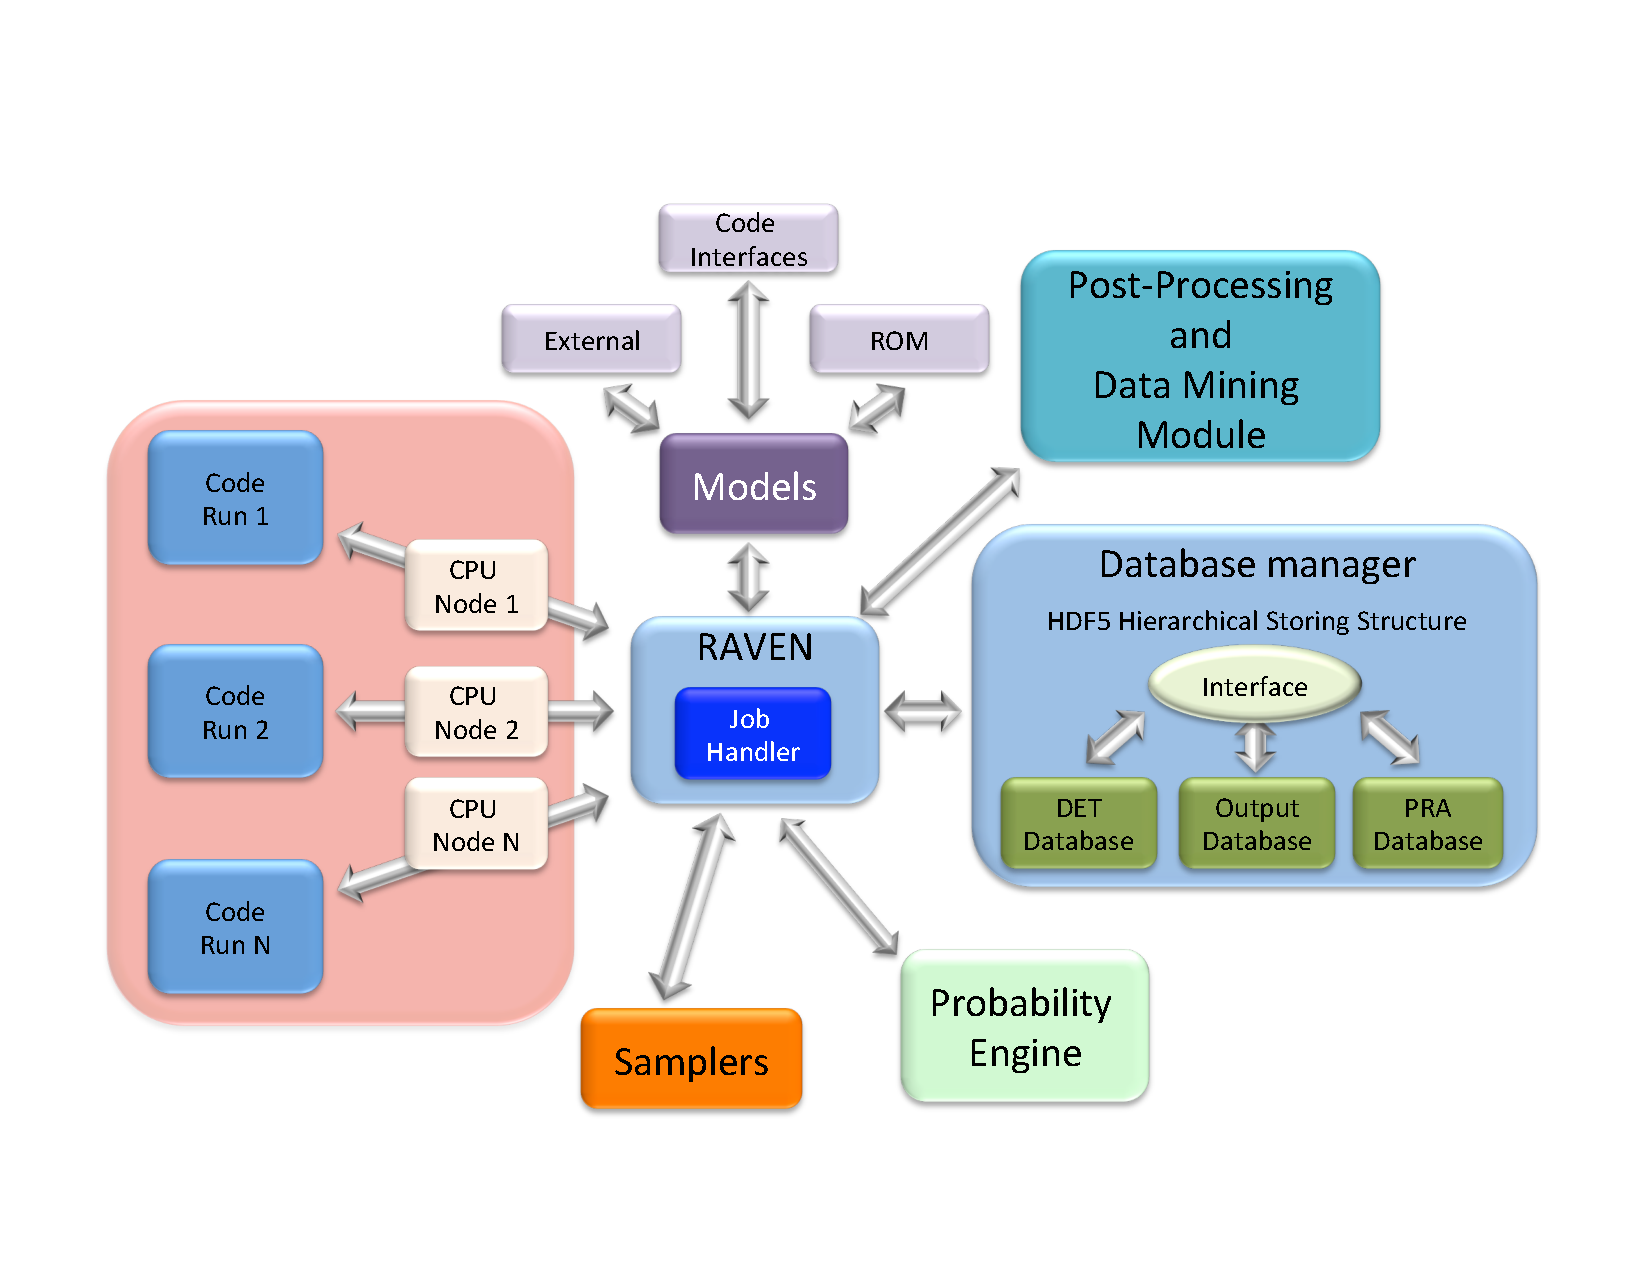
\includegraphics[scale=0.4]{raven.pdf}} 
    \caption{Overview of RAVEN statistical framework components}
    \label{fig:ravenScheme}
\end{figure}



\section*{References}

\bibliography{main}

\end{document}